\documentclass{sigchi}
% Arabic page numbers for submission.  Remove this line to eliminate
% page numbers for the camera ready copy
\pagenumbering{arabic}

% Load basic packages
\usepackage{balance}       % to better equalize the last page
\usepackage{graphics}      % for EPS, load graphicx instead 
\usepackage[T1]{fontenc}   % for umlauts and other diaeresis
\usepackage{txfonts}
\usepackage{mathptmx}
\usepackage[pdflang={en-US},pdftex]{hyperref}
\usepackage{color}
\usepackage{booktabs}
\usepackage{textcomp}
\usepackage{multirow}
\usepackage{hhline}
% Some optional stuff you might like/need.
\usepackage{microtype}        % Improved Tracking and Kerning
% \usepackage[all]{hypcap}    % Fixes bug in hyperref caption linking
\usepackage{ccicons}          % Cite your images correctly!
% option again before submitting your final document.
\usepackage{todonotes}

\def\plaintitle{SIGCHI Conference Proceedings Format}
\def\plainauthor{First Author, Second Author, Third Author,
  Fourth Author, Fifth Author, Sixth Author}
\def\emptyauthor{}
\def\plainkeywords{Authors' choice; of terms; separated; by
  semicolons; include commas, within terms only; required.}
\def\plaingeneralterms{Documentation, Standardization}

% llt: Define a global style for URLs, rather that the default one
\makeatletter
\def\url@leostyle{%
  \@ifundefined{selectfont}{
    \def\UrlFont{\sf}
  }{
    \def\UrlFont{\small\bf\ttfamily}
  }}
\makeatother
\urlstyle{leo}

% To make various LaTeX processors do the right thing with page size.
\def\pprw{8.5in}
\def\pprh{11in}
\special{papersize=\pprw,\pprh}
\setlength{\paperwidth}{\pprw}
\setlength{\paperheight}{\pprh}
\setlength{\pdfpagewidth}{\pprw}
\setlength{\pdfpageheight}{\pprh}

% Make sure hyperref comes last of your loaded packages, to give it a
% fighting chance of not being over-written, since its job is to
% redefine many LaTeX commands.
\definecolor{linkColor}{RGB}{6,125,233}
\hypersetup{%
  pdftitle={\plaintitle},
% Use \plainauthor for final version.
%  pdfauthor={\plainauthor},
  pdfauthor={\emptyauthor},
  pdfkeywords={\plainkeywords},
  pdfdisplaydoctitle=true, % For Accessibility
  bookmarksnumbered,
  pdfstartview={FitH},
  colorlinks,
  citecolor=black,
  filecolor=black,
  linkcolor=black,
  urlcolor=linkColor,
  breaklinks=true,
  hypertexnames=false
}

\makeatletter
\def\@copyrightspace{\relax}
\makeatother

% End of preamble. Here it comes the document.

\begin{document}

\title{FaceController: A Facial Feature Based Hands-free Interface for Computer Accessibility}

\numberofauthors{1}
\author{%
  \alignauthor{Yuwei Jiao\\
    \affaddr{University of Waterloo}\\
    \affaddr{Waterloo, On, Canada}\\
    \email{jyuwei@uwaterloo.ca}}\\
}

\maketitle

\begin{abstract}
% less than 150 words
% motivation
% summary of what the project is, what it will do, how it will be built.
% one or more contributions
FaceController is a face tracking based system that enables computer manipulations with simple facial expressions and enhances the computer and software accessibility, especially for the disabled.
Beyond a camera on the top of a computer monitor, there is no other hardware requirement of the system.
Supplemented by the power of face detection in OpenCV, FaceController provides a complete solution for building hands-free input system.
Foremost, FaceController allows people to move the cursor, click on buttons, control scroll bar, and type text via virtual keyboard in the screen with facial movements.  
Users can also set shortcuts for commands like opening/closing file or switching between panels with expressions like smiling or sad face.
FaceController has an innovative capability of sending system-wide click and keystroke signals.
Thus, it is conceivable that FaceController would provide another solution for the disabled to manipulate any software, and it could become the next generation input device. 
\end{abstract}

\keywords{face tracking, hands-free control, input device}

\section{Introduction}
% figure or caption is required with reference

\begin{figure}[h]
    \centering
    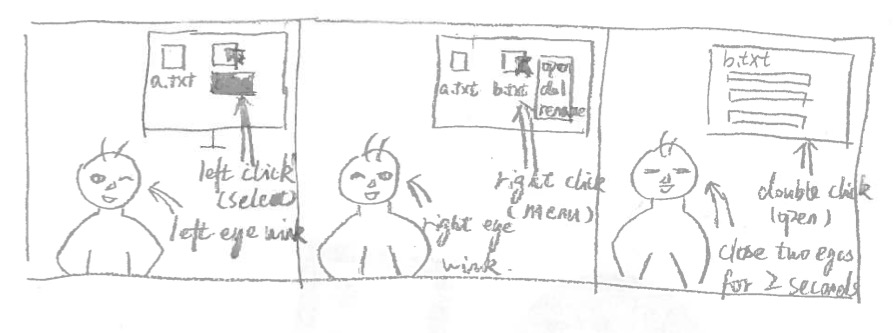
\includegraphics[width=0.9\columnwidth]{figures/sketch1}
    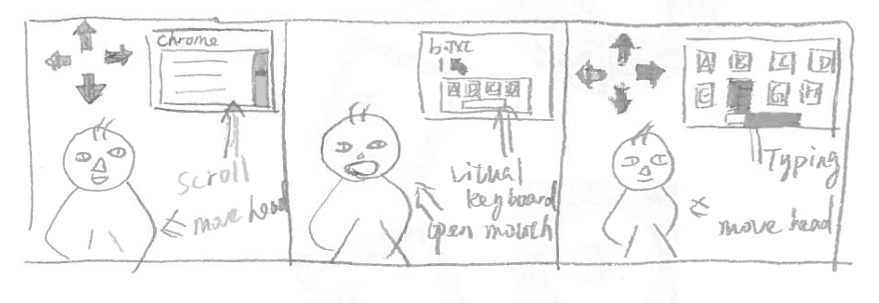
\includegraphics[width=0.9\columnwidth]{figures/sketch2}
    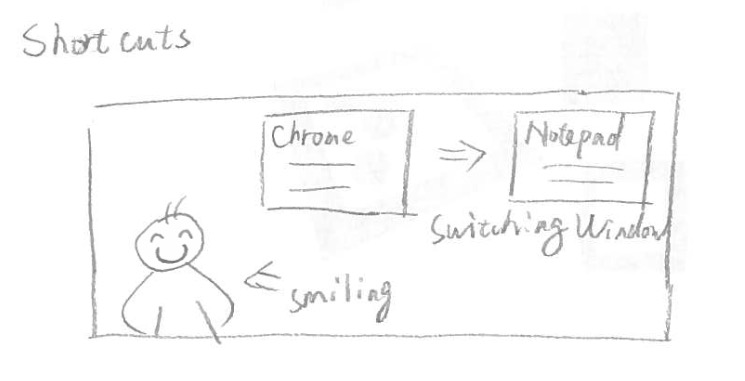
\includegraphics[width=0.9\columnwidth]{figures/sketch3}
    \caption{Sketch to illustrate FaceController}
    \label{fig:sketch}
\end{figure}

% problem context and motivation (why it's useful, what problem it solves)
The mouse and keyboard have been principal computer input devices for several years.
It is undeniable that they provide easy, accurate and sensible controls over computers.
However, input accessibility is far from solved.
Firstly, it is rather frustrating and exhausting if users need to switch between mouse and keyboard constantly for a period of time. 
Secondly, mouse and keyboard are not elegant solutions for direct manipulation as there remains a distance between hands and eyes.
Therefore users have to handle it carefully on what they do and what they see.
Thirdly, as input devices, mouse and keyboard are not accessible to the disabled.
As a result, traditional input devices somehow impair the accessibility and user experience, and also prevent people from realizing the full potential of computers.

% how your project idea is situated among related work
With the increase of machine power and decrease of camera cost, vision technology provides a way for a new generation input device. 
To be operational, vision based input interface requires to be "affordable, flexible, precise and robust"\cite{gorodnichy2004nouse}.
A few researchers have explored the possibility of using facial features to control computers and developed hands-free mouse replacements. 
However, most prototypes use the movement of eyes and nose, or markings on user's face to navigate the cursor.
These solutions do not take fully advantage of the information delivered by human's facial expressions.
There is still a large possible space unexplored.
Furthermore, the functionality of conventional input devices is weakened, for example, the ease of use and rapid response.

% expectation of project (what it is, what it will do, how it will be built)
In this paper, I present FaceController, a novel facial tracking based system that enables most software manipulations with basic human expressions (see Figure \ref{fig:sketch}).
The system-wide implementation allows users to move the cursor, click on buttons, control scroll bar and type characters directly via various facial expressions.
Each facial movement is bound with an input command in the system.
Currently FaceController is able to detect when users wink, raise either eyebrow, open their mouths and move heads around.
And it can also recognize combinations of facial movements, which enlarges expressing space and improves the flexibility.

% clear statement what the main research contributions 
In my implementation, I first applied a variety of face tracking algorithms in an attempt to find the optimal method in regard to accuracy and complexity.
Since the appearance of facial features differs among people, tracking performance varies among individuals.
Besides, enviromental factors, for example, lighting, might affect the performance as well.
Therefore it's necessary to take those factors into account.
Next step was to project from 3D facial movement to 2D cursor position.
FaceController provides three mouse cursor control modes: direct mode, joystick mode and differential mode.
And I will explore more on hands-free typing in the future.
Finally I present the discussions, as well as strengths and limitations of my prototype.

\begin{figure}[t]
    \centering
    \includegraphics[width=0.9\columnwidth]{figures/framework}
    \caption{The framework of FaceController}
    \label{fig:fig1}
\end{figure}

\begin{table}[t]
    \centering
    \begin{tabular}{ | p{0.4\columnwidth} | p{0.5\columnwidth} |}
    \hhline{==}
    \multicolumn{2}{|l|}{Movement} \\ \hhline{==}
    left / right eye wink & left / right button click \\ \hline
    close two eyes (> 2s) & double click \\ \hline
    open month & activate / deactivate virtual keyboard \\ \hline
    move closer to screen & activate scroll mode \\ \hline
    \multirow{3}{\hsize}{move head up / down / left / right} 
    & default mode: move the cursor\\ \cline{2-2}
    & scroll mode: scroll panel \\ \cline{2-2}
    & typing mode: typing alphabet \\ \hline
    raise left / right eyebrow & switch left / right windows \\ \hhline{==}
    \multicolumn{2}{|l|}{Expression} \\ \hhline{==}
    smiling face & zoom in \\ \hline
    sad face & zoom out \\ \hline
    angry face & return to desktop\\ \hhline{==}
    \end{tabular}
    \caption{Facial movements and expressions commands}
    \label{tab:table1}
\end{table}

\section{Related Work}
% under 1000 (1500) words; around ONE page
% no less than 15 related resources
% model the style and structure
% paper are discussed as related groups or categories, organized into subsections
% THREE questions:
% comprehensive in breadth and width; related theories have been investigated.
% still aspects of problem space not been solved or examined in detail
% your work is somehow different and novel
Assistive computer input systems that provide alternative methods to get controls of computers have been used and explored for a considerable period.
Besides using facial movements, people have tried to take advantages of other physical signals to communicate with computers effectively, for example, Keirn and Aunon suggested to control using brain-wave \cite{keirn1990man}.
Based on those ideas, people have tried to improve the recognition accuracy to communicate better \cite{pantic2000automatic} \cite{saragih2011deformable}.
In the field of facial expression recognition, several effective algorithms and methods have been published and applied for years.
And with the development of hardware and technology, computing efficiency has been improved greatly, which enlightens more complicated while accurate algorithms \cite{matsumoto2000algorithm} \cite{betke2002camera} \cite{morris2006facial} \cite{varona2008hands}.

\subsection{Methods}

\subsubsection{Electrooculography}
Electrooculography (EOG) is a technique for measuring the state of retina with pairs of electrodes placed near the eyes.
When eyes moving from one position to another, a possible difference occurs between the two electrodes and it becomes possible to estimate the potential eyes position and movement.
Kaufman et al developed an eye control system using EOG for the disabled \cite{kaufman1993eye} and indicated it was very inexpensive but applicable for most basic interaction devices.
The headphone prototype by Manabe et al also applied EOG and used Kalman filter to analyse the signals captured \cite{manabe2006full}. 
However, researchers indicate that EOG method is not accurate enough because of noisy signals.
People partly solved the problem using multiple pairs of electrodes.
After a training session of a few minutes, they indicated users could control several window functions naturally. 
However, the hardware requirements built a barrier for users.
Some users refused to take electrodes on face, and in some cases, the electrodes fall off, leading unpleasant user experiences.

In general, the two disadvantages of EOG method are extra hardware equipments and low manipulation accuracy in practice.

\subsubsection{Vision-based Methods}
Face detection using computer vision techniques has been explored thoroughly and applied to control mouse for years \cite{ware1987evaluation}.
Pantic and Rothkrantz gave an ideal system for facial expression detection, extraction, classification and analysis \cite{pantic2000automatic}, including stereo algorithm, color detector, eigenfaces and eigenfeatures.
This could be used as baseline in future studies. 

Stereo face tracking provides simple yet effective approach which is suitable for real-time processing \cite{matsumoto2000algorithm} \cite{saragih2011deformable} \cite{tu2007face} \cite{gorodnichy2004nouse}.
Matsumoto and Zelinsky's work included two cameras and re-constructed 3D facial feature model if any face found in both image streams \cite{matsumoto2000algorithm}.
Saragih et al proposed a method to improve the performance of stereo using deformable model fitting method \cite{saragih2011deformable}.
Driven by visual face tracking and 3D model, Tu et al developed a camera mouse system using only one camera as video input but able to retrieve 3D head motion parameters \cite{tu2007face}.
They designed three mouse control modes and compared the controllability under Windows XP.

PCA \cite{arai2010camera} \cite{saragih2011deformable} and Haar Cascades \cite{parmar2012facial} \cite{gorodnichy2004nouse} are also commonly used face recognition methods.


\subsection{Prototypes}
Man to machine communication through brain-wave processing is an interesting research topic for a long period of time.
Keirn and Aunon was interested in determine if it's possible to capture electrical activities in brain and monitor in the electroencephalography(EEG) \cite{keirn1990man}.
EEG measures voltage fluctuations with two electrodes place along user's scalp.
It's a typically noninvasive method.
Their work presented that it possible to capture and distinguish among various mental tasks with high degree of accuracy using EEG.
Therefore, translating these mental signals into a set of commands to external devices could be feasible. 
One of the significant extensions to this work is the real-time music notation developed by Eaton and Miranda \cite{eaton2013real}. 

Since last century, people start to focus on eye movements as a new method for computer input based on the observations that human direct visual attention by the movements of eyes. 
Colin \cite{ware1987evaluation} first carried out experiments to prove the feasibility of the eye tracker as a fast selection device for computers.
Takami et al developed a eye-control system for the disabled in 1995 \cite{takami1995computer}, which could be recognized as the first stage of smart home because users could control objects including TV, telephone and camera, etc.
Chen et al shared the similar idea of interaction with computers with special designed headphone and desk equipments \cite{chen1999new}, but the system was infrared-controlled. 
A wearable headphone-type gaze detector was proposed by Manabe et al in 2006 \cite{manabe2006full}.
With four EOG electrodes attached on the headphone near the eyes, the prototype could estimate gaze direction easily.
However, such headphones are not convenient and users would feel overwhelmed to wear then continuously.

Researchers are engaged in finding more natural methods to assist computer communication.
Combined head pose and gaze direction, several systems provide robust and accurate solutions to some degree \cite{matsumoto2000algorithm} \cite{arai2010camera} \cite{takami1995computer} \cite{magee2004eyekeys}.
Hornof and Caveder developed the system "EyeDraw" enabling children to draw with eyes \cite{hornof2005eyedraw}.
And a system based on gestures and movements helped doctors to control the position of laparoscope \cite{nishikawa2003face} 
Jota and Wigdor explored the design space of eyelid gestures systematically \cite{jota2015palpebrae} and they also developed prototypes for both computers and smart phones.
However, one problem for these systems is that, they only take the advantage of part of human facial movements (eyes).
Therefore the application fields are limited and the systems are not feasible in some cases.

In recent years, more facial movements and expressions have been take into considerations.
Gorodnichy and Roth proposed to use user's nose tip as mouse \cite{gorodnichy2004nouse}.
Camera Mouse has a developing history of more than ten years and keeps updating online \cite{betke2002camera} \cite{gips2000camera}.
It's a truly powerful and wonderful program.
Besides controlling and communicating through eyes, nose and head, it also allows user defined position on face to act as cursor.
And users can set parameters in GUI to adjust respond speed and smoothness. 
More experiments and evaluations were provided by Cloud et al \cite{cloud2002experiments}.

\section{Implementation}
% high level technical approach
% language, libraries, toolkits
% hardware requirement
% as detail as possible
% *sketch figures

\subsection{Framework}
The framework of FaceController is shown in Figure \ref{fig:fig1}.
No other hardware requirement is needed beyond a commodity computer with camera on the top.
There are at least three components in my system: the operating system to handle commands, the visual tracking module and the mouse/keystroke control module.
At present, FaceController is built on Mac OS Sierra 10.12.3 and uses the built-in webcam (720p FaceTime HD camera).

\subsection{Language, Libraries, Tookits}
FaceController is developed using Python 3.5.1 and takes the advantage of OpenCV (3.2.0) and Numpy (1.11.2) to handle image signals.
To control the mouse and keyboard programmatically, I adopt PyAutoGui (3.2.1) in FaceController.
PyAutoGui is a cross-platform Python module which can simulate moving, clicking, dragging the mouse and pressing, releasing and holding keys.
It even supports pressing keyboard hotkey combinations, which enables the functions of shortcuts in my implementation.
See {\url {http://pyautogui.readthedocs.io/en/latest/index.html}} for more information about PyAutoGui.

\begin{figure*}[h]
    \centering
    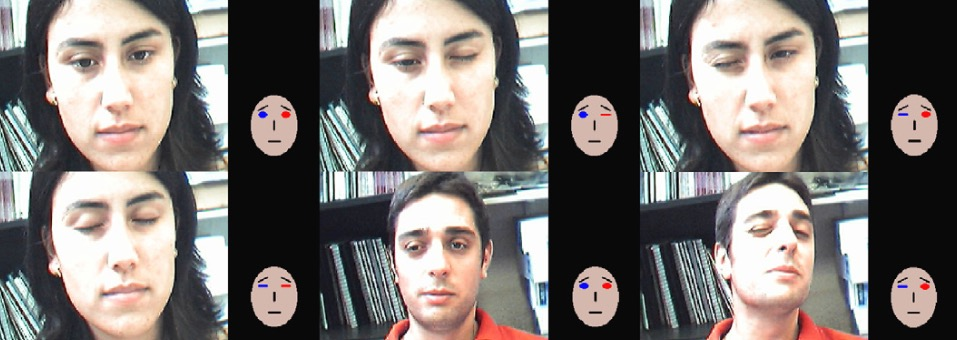
\includegraphics[width=1.8\columnwidth]{figures/winkdetection}
    \caption{Wink detection ~\protect\cite{varona2008hands}}
    \label{fig:fig3}
\end{figure*}

\begin{figure}[b]
    \centering
    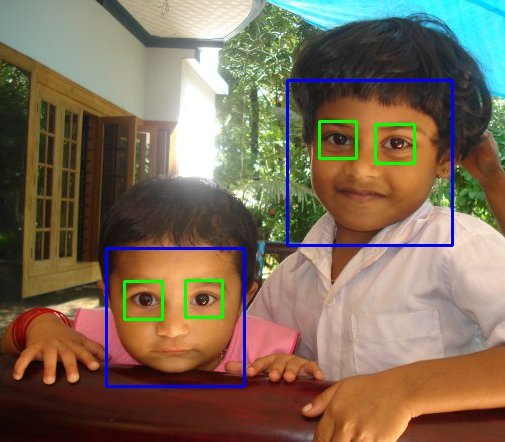
\includegraphics[width=0.9\columnwidth]{figures/facedetection}
    \caption{Face detection results using Haar Cascades in OpenCV}
    \label{fig:fig2}
\end{figure}

\subsection{Face Detection Algorithms}
Face Detection is the first step in the system (see Figure \ref{fig:fig2}).
There are several face detection algorithms to locate a human face in the screen.
Check out {\url {http://www.face-rec.org/algorithms/}}.
In my implementation, I applied the following techiniques:

\begin{itemize}
\setlength\itemsep{-0.2em}
\item {Principal Component Analysis (PCA)}
\item {Haar Feature-based Cascade Classifiers}
\item {...}
\end{itemize}

To be finished


\section{Discussion}
% what was done
% implications
% light evaluation on technical or user performance
% limitations of the technique

To be finished

\section{Future Work}
% advice and directions
% a brief description of a more formal user evaluation and technical evaluation that could been done

To be finished

% BALANCE COLUMNS
\balance{}

% REFERENCES FORMAT
% References must be the same font size as other body text.
\bibliographystyle{SIGCHI-Reference-Format}
\bibliography{CS889_YJ}

\end{document}
